\section{REALIS}\label{Sec:REALIS}
Wird bei Infineon von einem Kunden ein neues Produkt angefordert, oder entwickeln diese selber ein neues Produkt, so muss dieses zunächst getestet und qualifiziert werden, bevor es in Masse produziert werden kann. Mit Produkt ist dabei ein fertiger Chip, der auf einem Wafer hergestellt wurde, gemeint. Für diese Zuverlässigkeits- bzw. Qualitäts-Tests wurde bei Infineon eine Software mit dem Namen \gls{REALIS} entwickelt. Dieses System umfasst die komplette Planung und Dokumentation der Durchführung und Ergebnisse dieser Tests. Das System beinhaltet eine gleichnamige Datenbank, in denen alle wichtigen Information gespeichert werden.

\subsection{Projekt-Lebenszyklus}\label{Subsec:project-lifecycle}
Um ein neues Produkt zu testen, wird vom sogenannten \gls{QM} bei Infineon ein neues Projekt in \gls{REALIS} angelegt. Dieses befüllt er mit verschiedenen (Stress)-Tests, basierend auf vorhandenen Templates, die Arbeitsschritte (Operationen), Start- und Enddaten, Parameter der Operationen einzelner Tests und weitere Informationen enthalten. Dieser erste Schritt entspricht der obersten Reihe in Abbildung \ref{fig:realis-project-lifecycle} und bildet den Anfang eines REALIS Projekt-Lebenszyklus. 

Für jeden der folgenden weiteren Schritte wird in \gls{REALIS} der ``State``(Status) der Tests eines Projektes verändert und damit der Fortschritt dokumentiert. Dabei steht dieser zu Beginn immer auf  ``NEW`` und wird anschließend nach jedem der folgenden beschriebenen Schritte auf einen neuen ``State`` geändert (vgl. Abbildung \ref{fig:realis-project-lifecycle}, rechte Spalte). Welcher neue Zustand einem Test zugewiesen wird, wird dadurch entschieden, ob der beschriebene Schritt erfolgreich durchgeführt werden konnte.

Im zweiten Schritt des Lifecycles weist der \gls{QM} das Projekt, durch einen internen Mechanismus, einem ''State-Change'' des Projekts, einem sogenannten \todo{welchen RPT-Labor} \gls{RPT}-Labor zu. 

In einem \gls{RPT}-Labor validieren anschließend Mitarbeiter manuell die Richtigkeit der angelegten Tests und überprüfen daraufhin, ob sie die angelegten Stresstests des Projektes auch durchführen können. 
Für die Validierung der Tests werden die Stressparameter auf deren Sinnhaftigkeit überprüft. Die Frage der Durchführbarkeit hängt davon ab, ob im zugewiesenen \gls{RPT}-Labor Maschinen vorhanden sind, die in der Lage sind, die geforderten Stressoperationen auszuführen und die festgelegten Stressparameter einzuhalten. Zudem müssen diese Maschinen betriebsbereit sein – also weder in Benutzung noch außer Betrieb.

Diese Prüfungen bezeichnen den aktuellen technischen Feasibility Check, dessen Ergebnisse in \gls{REALIS} dokumentiert werden.
Falls für einige Operationen bzw. Tests keine gültigen Maschinen vorhanden sind, werden diese Tests an andere \gls{RPT}-Labore delegiert. Dadurch müssen die zu testenden Produkte jedoch von einem Labor zum anderen transportiert werden, was aufgrund der weltweiten Verteilung viel Zeit in Anspruch nehmen kann.

\begin{figure}[!h]
    \centering
    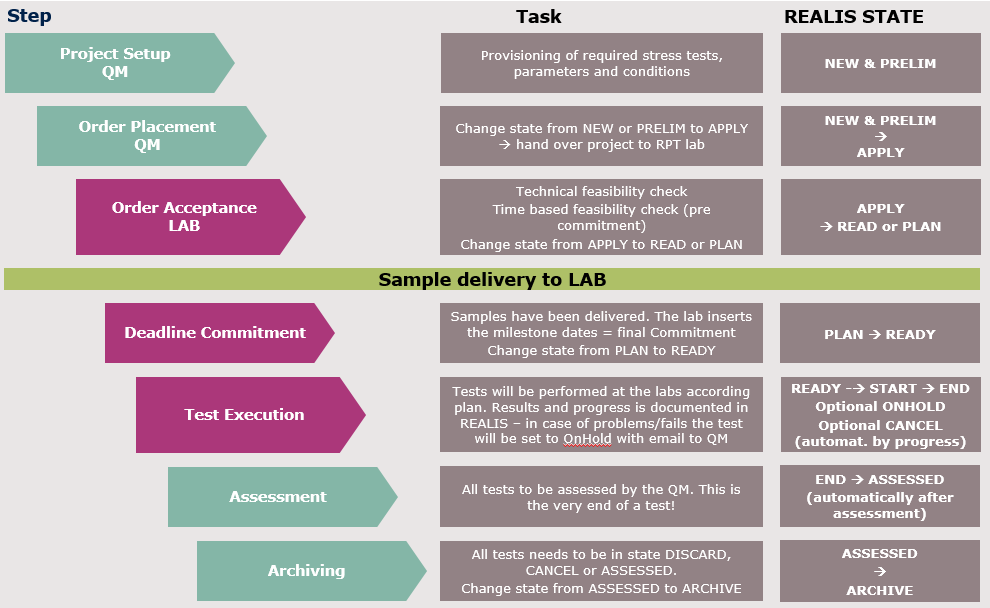
\includegraphics[width=1\textwidth]{bilder/realis-project-lifecycle.png}
    \caption{REALIS Project Lifecycle \cite{REALISWikiIntern}}
    \label{fig:realis-project-lifecycle}
\end{figure}

Anschließend wird ein ''Sample'', also eine kleine Stückzahl des Produktes, zum beauftragten \gls{RPT}-Labor geschickt. Dieses wird in der Fachsprache auch als \textit{Test lot}, oder zu Deutsch: \textit{Test-Los} bzw. nur \gls{los} bezeichnet. Die Stückzahl wird dabei in \gls{REALIS} dokumentiert. Die  Daten der Testoperation werden dann final festgelegt und der Test-Status wird geändert.

Daraufhin erfolgt die planmäßige Durchführung der einzelnen Operationen der Stresstests. Dabei werden der Fortschritt und die Ergebnisse von Labor-Mitarbeitern, sogeannten \glspl{operator}, in \gls{REALIS} dokumentiert. Treten während der Stresstests Probleme oder Fehler auf, werden diese an den \gls{QM} weitergeleitet, der anschließend über das weitere Vorgehen entscheidet.

Nachdem alle Tests vollständig durchgeführt und dokumentiert worden sind, muss der \gls{QM} die Ergebnisse prüfen und bewerten. Zum Schluss werden die Tests dann archiviert, wobei aus Gewährleistungsgründen die Chips und Testergebnisse 16 Jahre aufbewahrt werden müssen, womit der Projekt-Lebenszyklus beendet ist.

\subsection{Architektur und Technologie}
Das ursprüngliche Frontend von REALIS war eine Windows-Desktop-Applikation, die sowohl vom \gls{RPT}-Labor-Mitarbeiter als auch vom \gls{QM} genutzt wurde. Im Zuge einer Modernisierung wird das System schrittweise zu einer Web-Applikation migriert. Zeitgleich erfolgt eine Aufteilung in zwei separate Anwendungen, eine für den \gls{QM} und eine für den \gls{operator}, um die Geschäftsprozesse zu vereinfachen und die Nutzerfreundlicheit zu verbesssern.

Abbildung \ref{fig:realis-komponentendiagramm} zeigt die aktuelle Systemarchitektur in Form eines Komponentendiagramms. Im Backend (grün dargestellt) kommuniziert der \texttt{REALIS-Server} über eine \texttt{DataAccess}-Schnittstelle direkt mit der zentralen \texttt{REALIS-Datenbank}, welche auf Oracle basiert. Der \texttt{REALIS-Server} stellt die Geschäftslogik (Business-Layer) bereit und wird über eine \texttt{REST-API} von den Frontends genutzt.

\begin{figure}[!h]
    \centering
    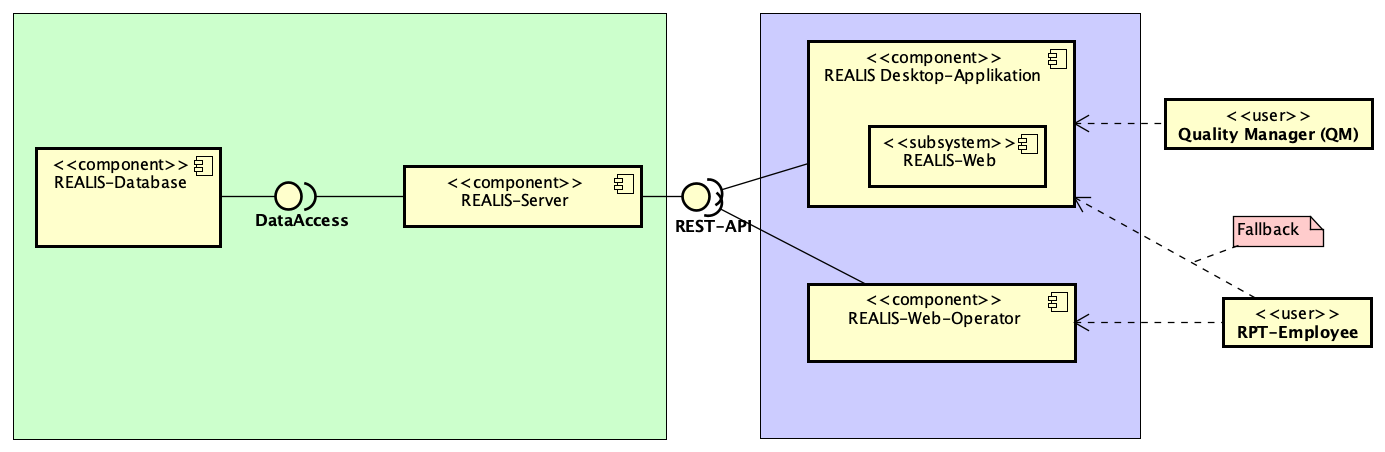
\includegraphics[width=1\textwidth]{bilder/REALIS-Komponentendiagramm.png}
    \caption{REALIS Komponentendiagramm}
    \label{fig:realis-komponentendiagramm}
\end{figure}

Das Frontend besteht aus zwei Hauptkomponenten (blau dargestellt):
\begin{enumerate}
    \item \textbf{REALIS-Desktop-Applikation:} \\
Die ursprüngliche Desktop-Anwendung, die sukzessive durch die Integration von neuen Web-Funktionalitäten modernisiert wird. Diese Web-Module, die mit dem Framework Angular entwickelt werden, sind als Subsystem (\texttt{REALIS-Web}) innerhalb der Desktop-Applikation eingebettet. Dieses System steht sowohl dem \gls{QM} als auch dem \gls{RPT}-Labor-Mitarbeiter zur Verfügung. Langfristig soll der \gls{RPT}-Labor-Mitarbeiter jedoch keinen Zugriff mehr darauf haben.

\item \textbf{REALIS-Web-Operator-System:} \\
Eine eigenständige Web-Applikation, die speziell für die Anforderungen des \gls{RPT}-Labors entwickelt wird. Diese Anwendung befindet sich noch in der Entwicklung, wird jedoch bereits für einige Aufgaben eingesetzt. Für nicht implementierte Funktionen muss der \gls{RPT}-Mitarbeiter vorübergehend auf die alte Desktop-Applikation ausweichen. Zusätzlich ist geplant, das \texttt{REALIS-Web-Operator-System} als native iOS-App für mobile Apple-Geräte (z. B. iPads, iPhones) bereitzustellen. Die Verwendung von Angular ermöglicht dabei eine plattformübergreifende Entwicklung, die sowohl als Web-App als auch als native App funktioniert.
\end{enumerate}

Das Diagramm \ref{fig:realis-komponentendiagramm} verdeutlicht die Trennung zwischen Backend und Frontend sowie die unterschiedlichen Nutzerrollen (\gls{QM} und \gls{RPT}-Employee), die spezifische Zugriffsrechte auf die jeweiligen Systeme haben.


\subsection{Weitere Funktionen und Statistiken}
Neben der Möglichkeit, Qualitätstests (Reliability-Tests) anzulegen, bietet \gls{REALIS} eine Vielzahl zusätzlicher Funktionen, die dazu beitragen, Prozesse effizienter zu gestalten und Engpässe zu vermeiden. So unterstützt das System beispielsweise die Planung individueller Laborkapazitäten, wodurch unnötige Investitionen vermieden und vorhandene Ressourcen optimal genutzt werden können. Darüber hinaus ermöglicht \gls{REALIS} die Referenzierung bereits durchgeführter Testergebnisse, um redundante Tests zu vermeiden und Zeit sowie Kosten zu sparen.

Nach Abschluss eines Tests können in \gls{REALIS} automatisch benötigte Ergebnisberichte generiert werden – sowohl für den Kunden als auch für das \gls{RPT}-Labor. Dies erleichtert die Dokumentation und erhöht die Effizienz im Testmanagement.

Seit 2001 ist \gls{REALIS} im Einsatz und wird derzeit von etwa 4.300 aktiven Nutzern verwendet. Das System findet Anwendung in 101 \gls{RPT}-Laboren in 17 Ländern. Aktuell verwaltet \gls{REALIS} rund 270.000 Projekte mit etwa 1,9 Millionen Stresstests \cite{REALISPowerPointIntern}.